\chapter{Ánalisis de la situación}

El principal objetivo del dataset de Gas Drift de UCI es proporcionar un bechmark donde probar las diferentes soluciones
y algoritmos para afrontar el problema de la deriva de sensores de gas, también conocidos como narices electrónicas.

En la Figure \ref{fig:sensorphoto} \cite{Zhao2019} podemos ver la disposición del sistema de adquisición para construir el dataset que finalmente está disponible en UCI.

El gas pasa por la placa de adquisición, donde las señales temporales generadas por cada sensor (Figura \ref{fig:sensor_response}) se descomponen en dos componentes de continua y 6 componentes de transitorio, 3 caracterizando la entrada del gas, y 3 caracterizando la salida. En la Figura \ref{fig:tabfeatures} se resumen estas carateristicas. Para más detalle del significado de las componentes consultar \cite{Vergara2011}

Por tanto el dataset proporcionado caracteriza a cada gas con 128 componentes obtenidas de los diferentes sensores, 1 componente que especifica la concentración presente de ese gas en la medición, y el batch al que pertenece la medición, es decir,
en qué meses se realizó. En total tendríamos 2 variables objetivo (gas y concentración), 128 características, y una componente temporal (batch id).

Esto presenta un reto para entrenar un algoritmo de clasificación, por varios motivos:
\begin{itemize}
\item Para un mismo gas, los sensores capturaran diferentes respuestas para diferentes concentraciones
\item Una medición de un gas a una concentración dada, no será igual en los primeros meses de medición que en los últimos, debido a la deriva del sensor.
\item Se han usado 4 tipos de sensores, y dentro de cada tipo se usaron 4 calibraciones diferentes \cite{Zhao2019} por lo que podría darse la situación de que algún sensor no sea capaz de detectar el paso del gas, o se vea saturado, dando una medición no valida para clasificar.
\end{itemize}

En este trabajo primero comprobaremos que
\begin{itemize}
	\item Existe esta deriva de los sensores. Comparación de la misma señal a lo largo de los meses.
	\item Esta deriva afecta a los modelos de clasificación. Modelo de clasificación muy sencillo con una red neuronal secuencial.
	\item Existe correlación entre las mediciones de los 16 sensores, ya que se trata de 16 mediciones del mismo fenómeno. Es más, las 8 componentes la descomposición propuesta de la señal, no son independientes entre sí.
\end{itemize}

\begin{figure}
	\centering
	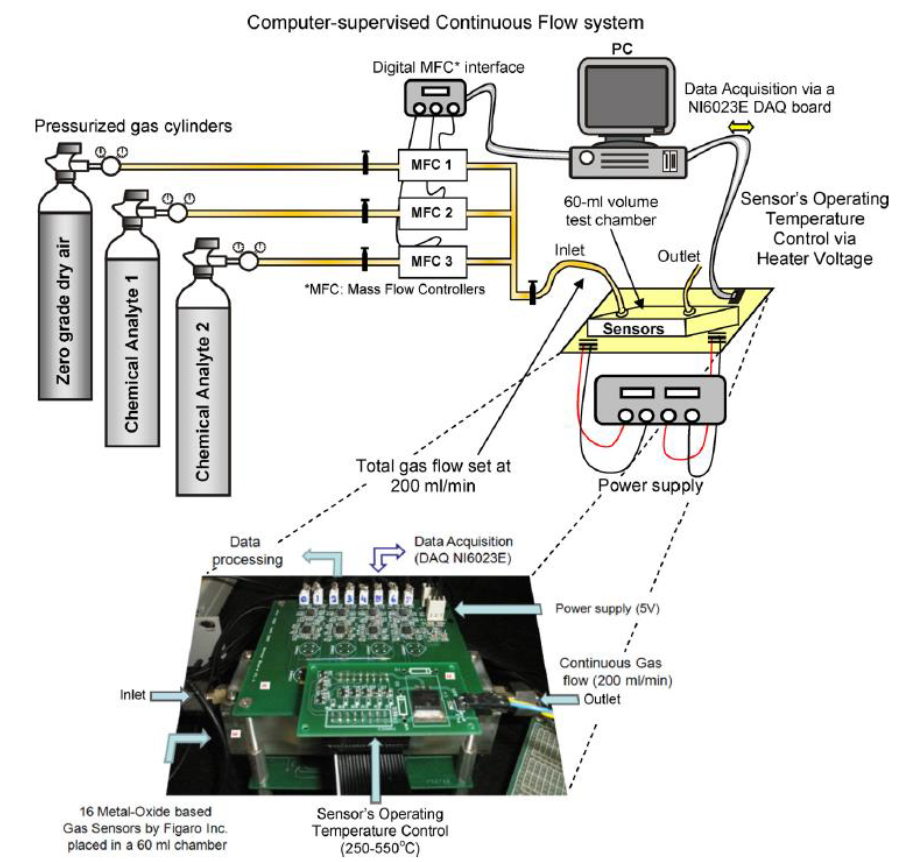
\includegraphics[width=0.95\linewidth]{../py_imgs/sensor_photo}
	\caption[Esquema de sistema de adquisición de datos]{Esquema del sistema de adquisición, donde pueden verse los 16 sensores de gas Figaro.}
	\label{fig:sensorphoto}
\end{figure}

\begin{figure}
	\centering
	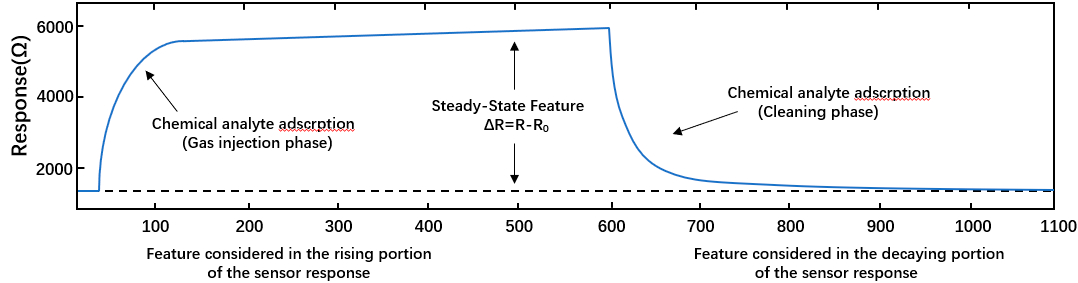
\includegraphics[width=0.95\linewidth]{../py_imgs/sensor_response}
	\caption[Respuesta del sensor]{Información típica de la respuesta del sensor. Respuesta típica de una sustancia química a base de óxido metálico sensor a 30ppmv de acetaldehído. La curva muestra las tres fases de una medición: línea de base medición (realizada con aire puro), medición del gas de prueba (cuando se inyecta el analito químico, en forma de gas, a la cámara de prueba) y fase de recuperación (durante la cual el sensor se expone nuevamente a aire puro; el tiempo de recuperación suele ser mucho más largo que la inyección de gas\protect\cite{Vergara2011}}
	\label{fig:sensor_response}
\end{figure}

\begin{figure}
	\centering
	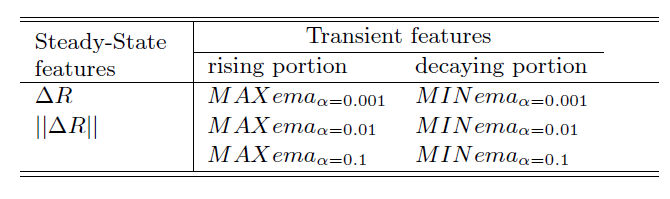
\includegraphics[width=0.95\linewidth]{../py_imgs/tab_features}
	\caption[Descomposición de las señales temporales]{Descripción de la descomposición de las señales temporales generadas por los sensores. Más información en \protect\cite{Vergara2011}}
	\label{fig:tabfeatures}
\end{figure}
